\subsection*{Estabilidad de resultados}

Se realizaron 100 ejecucciones para cada par de función y método de optimización partiendo de un punto aleatorio dado por la distribución normal con media 0 y desviación 10 (ecuación \ref{eq:initial_point}).

\begin{equation}
    x_0 =  \mathcal{N}(\mu=0;\sigma=10)
    \label{eq:initial_point}
\end{equation}

En la figura \ref{fig:quadracic_function} se muestra el valor de la función y la norma del gradiente para la mejor iteración para cada método con la función cuadrática con matriz diagonal.

\begin{figure}[H]
    \centering
    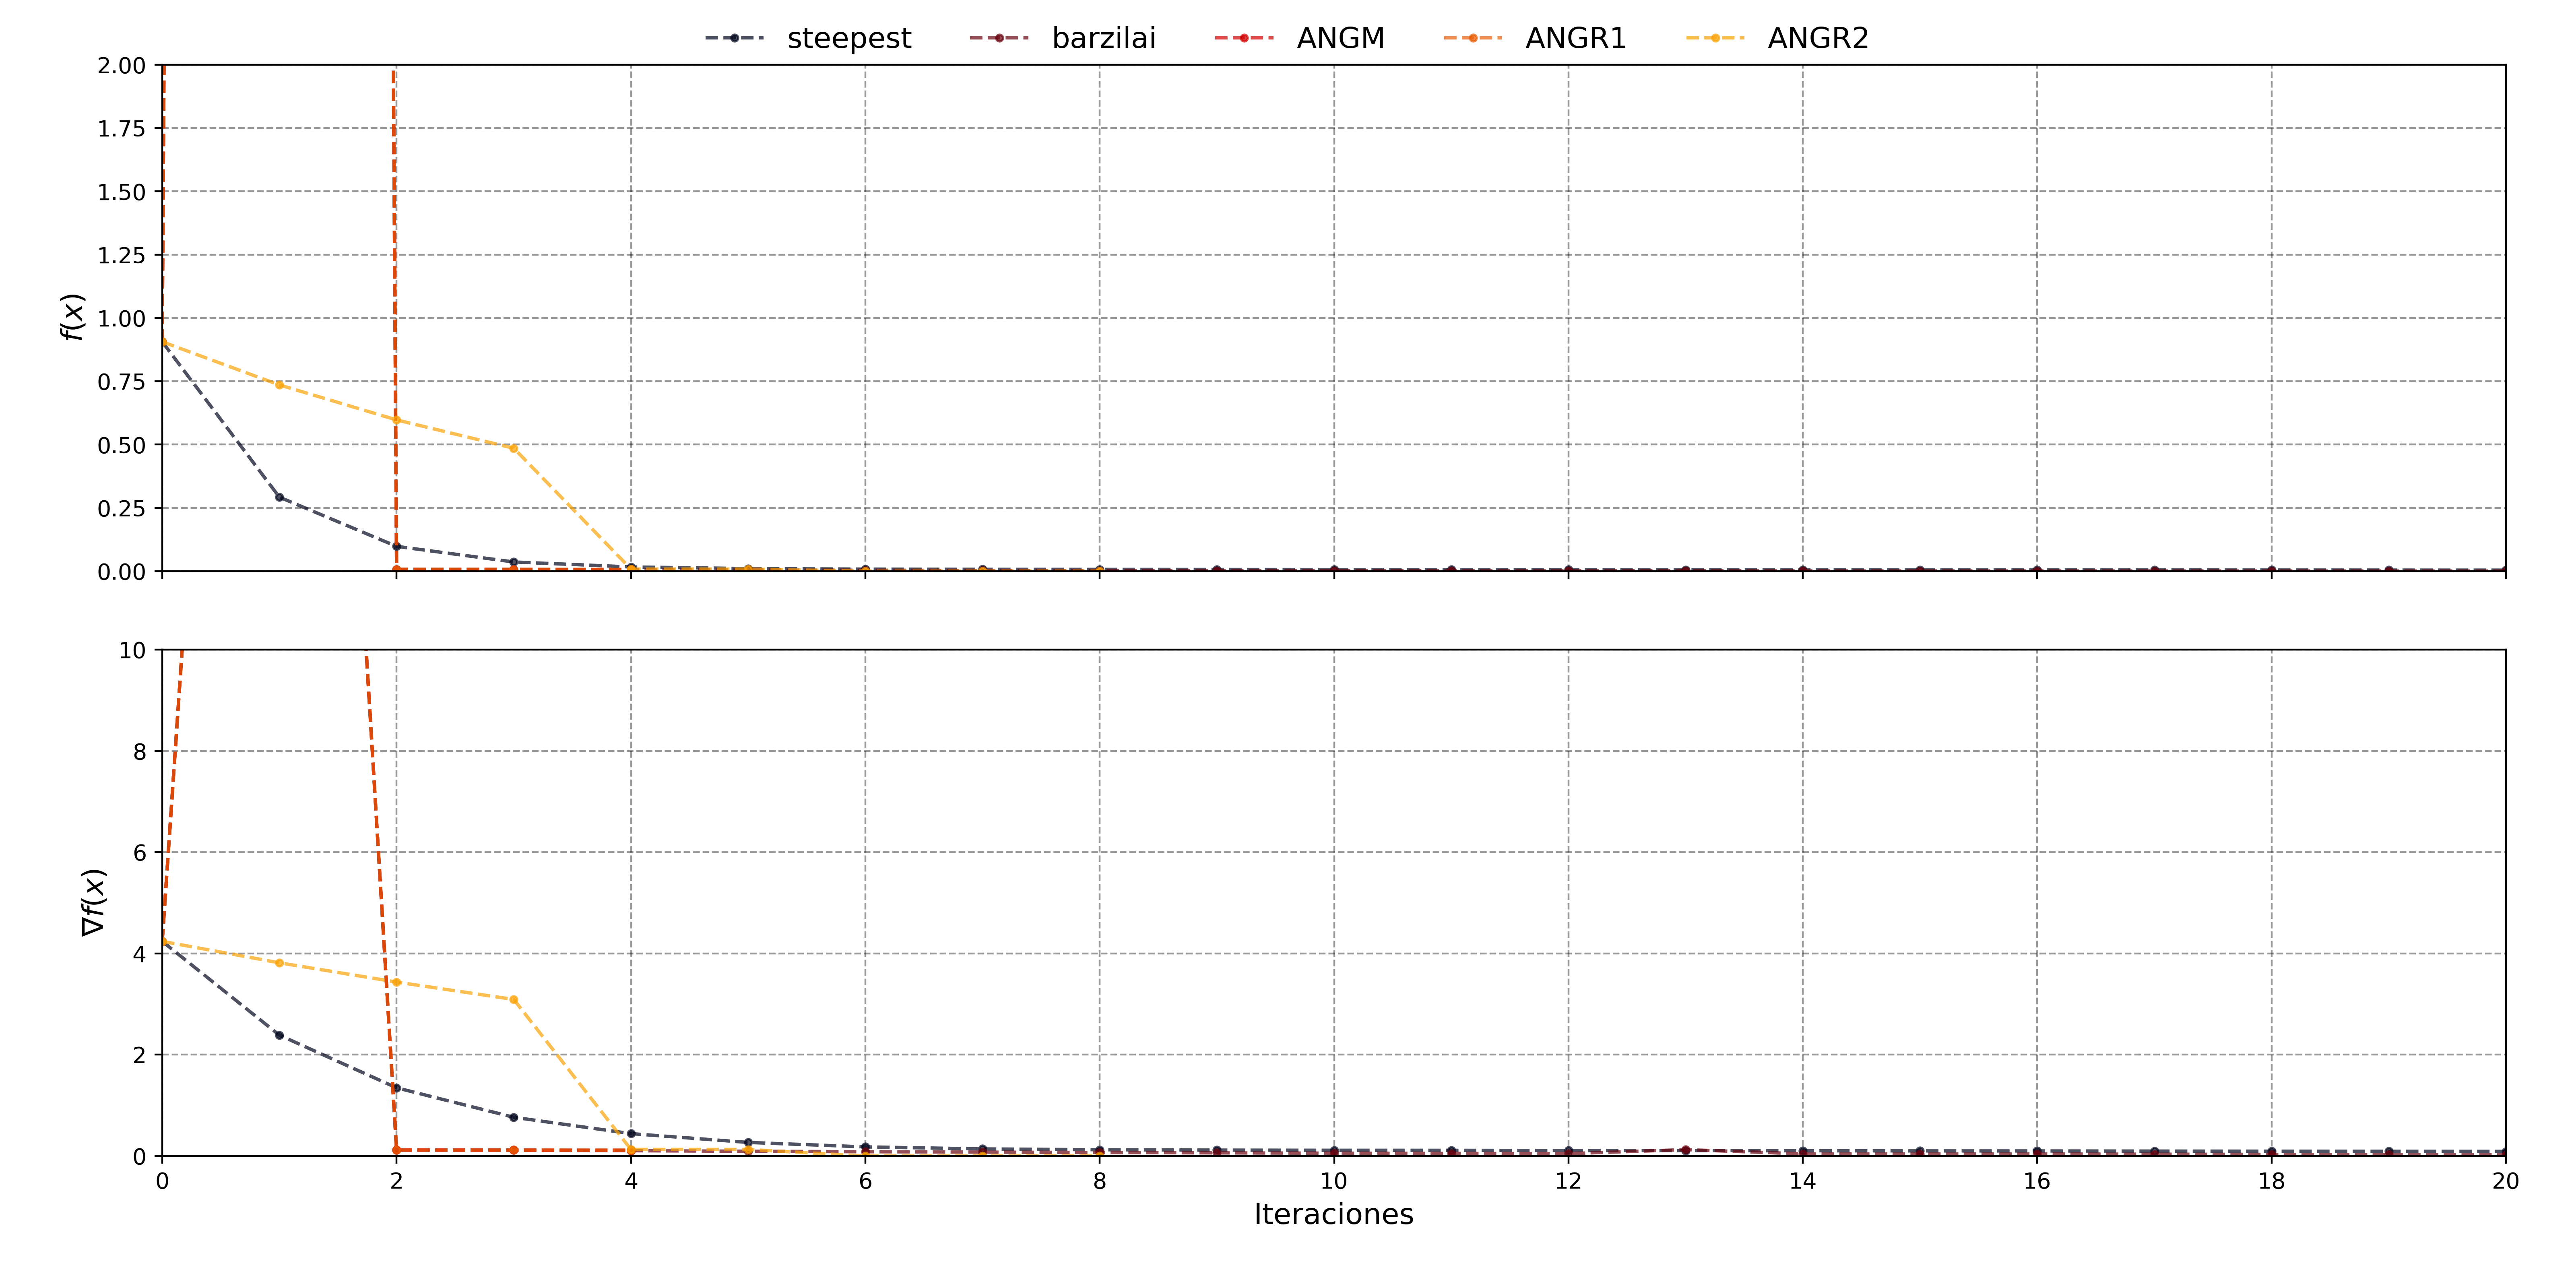
\includegraphics[width=17cm]{graphics/function/quadratic.png}
    \caption{Valor de la función y norma del gradiente en cada iteración de la mejor ejecución de cada método de optimización de la función cuadrática con matriz diagonal.}
    \label{fig:quadracic_function}
\end{figure}

Se realizó el mismo procedimiento con la función de Rosembrock. En la figura \ref{fig:rosembrock_function} se muestra el resultado del valor de la función y norma del gradiente para la mejor iteración de cada método.

\begin{figure}[H]
    \centering
    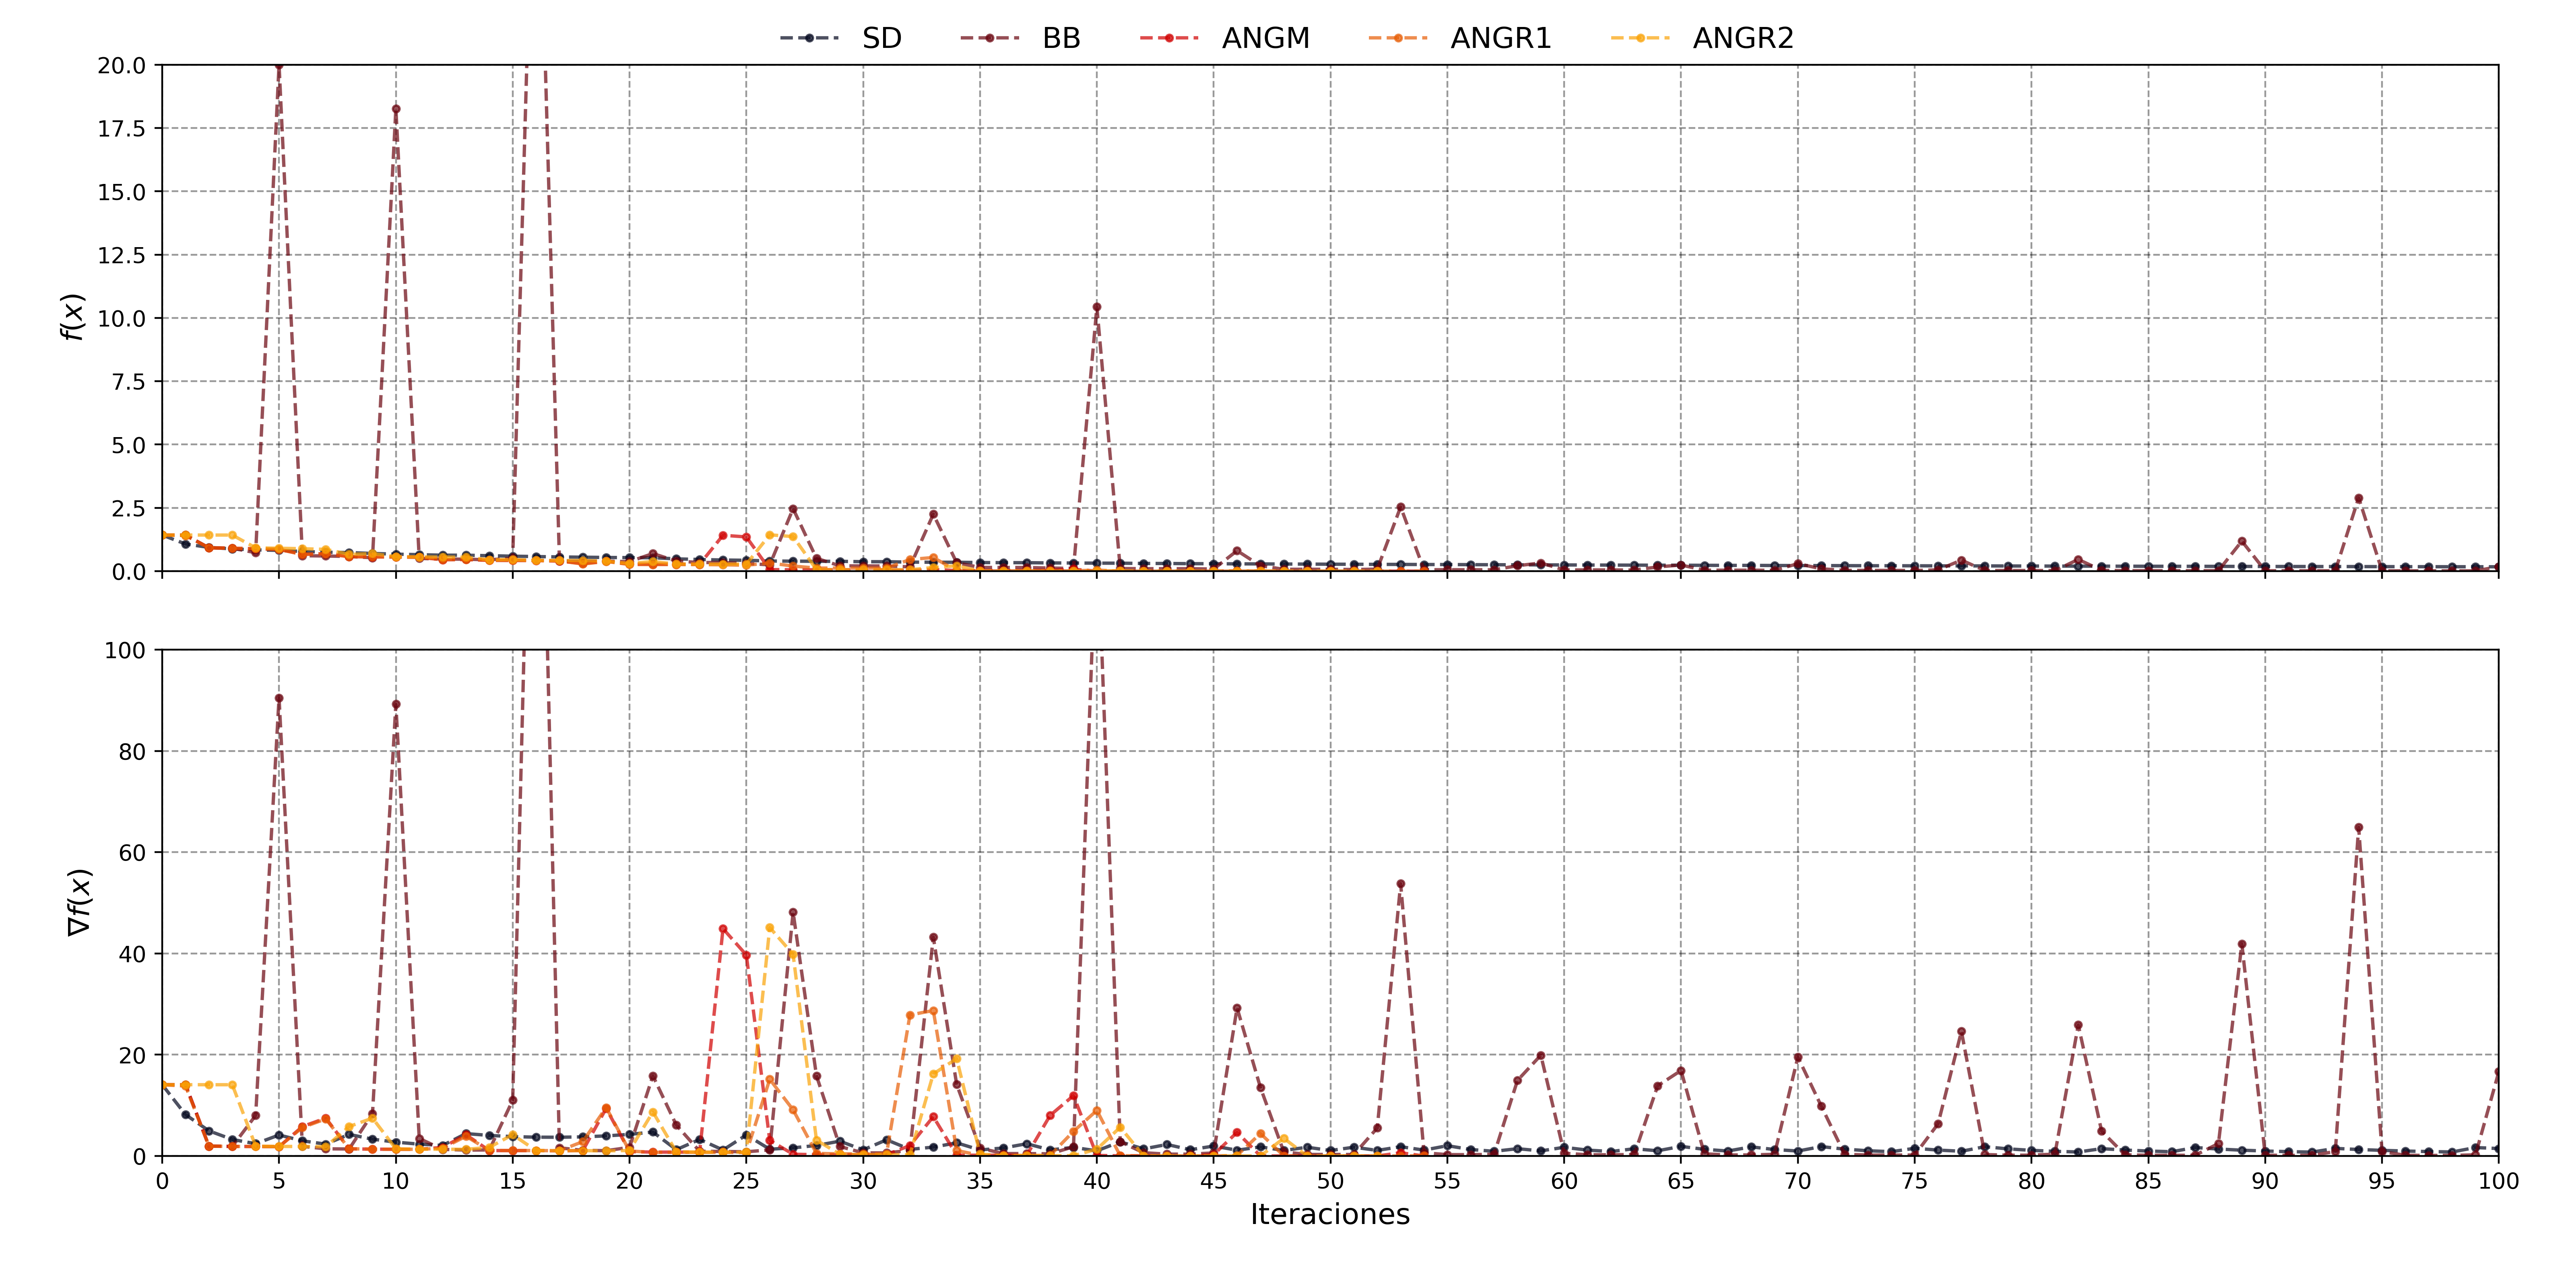
\includegraphics[width=17cm]{graphics/function/rosembrock.png}
    \caption{Valor de la función y norma del gradiente en cada iteración de la mejor ejecución de cada método de optimización de la función de Rosembrock con matriz diagonal.}
    \label{fig:rosembrock_function}
\end{figure}

En las tablas \ref{table:mean} y \ref{table:deviation} se muestran las medias y desviaciones estandar para el valor de la función y norma de gradiente en el punto óptimio y el número de iteraciones realizadas por cada método y función.

\begin{table}[H]
    \changefontsizes{10pt}
    \centering
    \begin{tabular}{llrrrrr}
        \hline                                                                                                           \\
        \textbf{Función} & \textbf{Valor} & \textbf{SD}  & \textbf{BB} & \textbf{ANGM} & \textbf{ANGR1} & \textbf{ANGR2} \\[0.1cm]\hline
        \\
                         & Función        & 0.000000     & 0.000000    & 0.000000      & 0.000000       & 0.000000       \\[0.25cm]
        Lambda           & Gradiente      & 0.000001     & 0.000001    & 0.000001      & 0.000001       & 0.000001       \\[0.25cm]
                         & Iteraciones    & 7764.810000  & 2770.340000 & 252.430000    & 289.490000     & 255.830000     \\[0.25cm]\hline
        \\
                         & Función        & 0.000000     & 0.000000    & 0.000000      & 0.000000       & 0.000000       \\[0.25cm]
        Cuadrática       & Gradiente      & 0.000001     & 0.000001    & 0.000000      & 0.000000       & 0.000000       \\[0.25cm]
                         & Iteraciones    & 713.000000   & 1531.230000 & 5.240000      & 7.360000       & 9.700000       \\[0.25cm]\hline
        \\
                         & Función        & 4.161332     & 42.245667   & 0.000000      & 0.000000       & 0.000000       \\[0.25cm]
        Rosembrock       & Gradiente      & 0.566027     & 45.446672   & 0.000000      & 0.000000       & 0.000000       \\[0.25cm]
                         & Iteraciones    & 10000.000000 & 1603.210000 & 68.840000     & 70.170000      & 67.150000      \\[0.25cm]\hline
        \\
                         & Función        & 0.000000     & 3.158103    & 5.070144      & 4.561704       & 8.428735       \\[0.25cm]
        Wood             & Gradiente      & 0.000004     & 0.000001    & 0.000000      & 0.000000       & 0.000000       \\[0.25cm]
                         & Iteraciones    & 9428.690000  & 1806.430000 & 360.360000    & 292.430000     & 199.210000     \\[0.25cm]\hline
    \end{tabular}
    \caption{Media de las 100 ejecucciones partiendo de puntos aleatorios.}
\end{table}

\begin{table}[H]
    \changefontsizes{11pt}
    \centering
    \begin{tabular}{llrrrrr}
        \hline                                                                                                          \\
        \textbf{Función} & \textbf{Valor} & \textbf{SD} & \textbf{BB} & \textbf{ANGM} & \textbf{ANGR1} & \textbf{ANGR2} \\[0.1cm]\hline
        \\
                         & Función        & 0.000000    & 0.000000    & 0.000000      & 0.000000       & 0.000000       \\[0.25cm]
        Lambda           & Gradiente      & 0.000000    & 0.000000    & 0.000000      & 0.000000       & 0.000000       \\[0.25cm]
                         & Iteraciones    & 612.385412  & 209.340437  & 32.553066     & 28.338322      & 25.043016      \\[0.25cm]\hline
        \\
                         & Función        & 0.000000    & 0.000000    & 0.000000      & 0.000000       & 0.000000       \\[0.25cm]
        Cuadrática       & Gradiente      & 0.000000    & 0.000000    & 0.000000      & 0.000000       & 0.000000       \\[0.25cm]
                         & Iteraciones    & 43.810658   & 96.111137   & 1.198652      & 1.856030       & 2.886751       \\[0.25cm]\hline
        \\
                         & Función        & 14.244453   & 393.585673  & 0.000000      & 0.000000       & 0.000000       \\[0.25cm]
        Rosembrock       & Gradiente      & 1.357743    & 396.058464  & 0.000000      & 0.000000       & 0.000000       \\[0.25cm]
                         & Iteraciones    & 0.000000    & 1867.607211 & 17.317429     & 20.596192      & 14.927011      \\[0.25cm]\hline
        \\
                         & Función        & 0.000000    & 10.092718   & 12.223427     & 11.860350      & 14.404998      \\[0.25cm]
        Wood             & Gradiente      & 0.000019    & 0.000000    & 0.000000      & 0.000000       & 0.000000       \\[0.25cm]
                         & Iteraciones    & 465.597882  & 633.528762  & 190.558643    & 204.762156     & 119.763512     \\[0.25cm]\hline
    \end{tabular}
    \caption{Desviaciones estandar de las 100 ejecucciones partiendo de puntos aleatorios.}
    \label{table:deviation}
\end{table}